% Options for packages loaded elsewhere
\PassOptionsToPackage{unicode}{hyperref}
\PassOptionsToPackage{hyphens}{url}
\PassOptionsToPackage{dvipsnames,svgnames,x11names}{xcolor}
%
\documentclass[
  12pt,
  a4paper,
]{article}

\usepackage{amsmath,amssymb}
\usepackage{setspace}
\usepackage{iftex}
\ifPDFTeX
  \usepackage[T1]{fontenc}
  \usepackage[utf8]{inputenc}
  \usepackage{textcomp} % provide euro and other symbols
\else % if luatex or xetex
  \usepackage{unicode-math}
  \defaultfontfeatures{Scale=MatchLowercase}
  \defaultfontfeatures[\rmfamily]{Ligatures=TeX,Scale=1}
\fi
\usepackage{lmodern}
\ifPDFTeX\else  
    % xetex/luatex font selection
    \setmainfont[]{Latin Modern Roman}
    \setsansfont[]{Latin Modern Roman}
\fi
% Use upquote if available, for straight quotes in verbatim environments
\IfFileExists{upquote.sty}{\usepackage{upquote}}{}
\IfFileExists{microtype.sty}{% use microtype if available
  \usepackage[]{microtype}
  \UseMicrotypeSet[protrusion]{basicmath} % disable protrusion for tt fonts
}{}
\usepackage{xcolor}
\usepackage[top=2.5cm,bottom=2.5cm,left=2.5cm,right=2.5cm]{geometry}
\setlength{\emergencystretch}{3em} % prevent overfull lines
\setcounter{secnumdepth}{5}
% Make \paragraph and \subparagraph free-standing
\makeatletter
\ifx\paragraph\undefined\else
  \let\oldparagraph\paragraph
  \renewcommand{\paragraph}{
    \@ifstar
      \xxxParagraphStar
      \xxxParagraphNoStar
  }
  \newcommand{\xxxParagraphStar}[1]{\oldparagraph*{#1}\mbox{}}
  \newcommand{\xxxParagraphNoStar}[1]{\oldparagraph{#1}\mbox{}}
\fi
\ifx\subparagraph\undefined\else
  \let\oldsubparagraph\subparagraph
  \renewcommand{\subparagraph}{
    \@ifstar
      \xxxSubParagraphStar
      \xxxSubParagraphNoStar
  }
  \newcommand{\xxxSubParagraphStar}[1]{\oldsubparagraph*{#1}\mbox{}}
  \newcommand{\xxxSubParagraphNoStar}[1]{\oldsubparagraph{#1}\mbox{}}
\fi
\makeatother


\providecommand{\tightlist}{%
  \setlength{\itemsep}{0pt}\setlength{\parskip}{0pt}}\usepackage{longtable,booktabs,array}
\usepackage{calc} % for calculating minipage widths
% Correct order of tables after \paragraph or \subparagraph
\usepackage{etoolbox}
\makeatletter
\patchcmd\longtable{\par}{\if@noskipsec\mbox{}\fi\par}{}{}
\makeatother
% Allow footnotes in longtable head/foot
\IfFileExists{footnotehyper.sty}{\usepackage{footnotehyper}}{\usepackage{footnote}}
\makesavenoteenv{longtable}
\usepackage{graphicx}
\makeatletter
\def\maxwidth{\ifdim\Gin@nat@width>\linewidth\linewidth\else\Gin@nat@width\fi}
\def\maxheight{\ifdim\Gin@nat@height>\textheight\textheight\else\Gin@nat@height\fi}
\makeatother
% Scale images if necessary, so that they will not overflow the page
% margins by default, and it is still possible to overwrite the defaults
% using explicit options in \includegraphics[width, height, ...]{}
\setkeys{Gin}{width=\maxwidth,height=\maxheight,keepaspectratio}
% Set default figure placement to htbp
\makeatletter
\def\fps@figure{htbp}
\makeatother
% definitions for citeproc citations
\NewDocumentCommand\citeproctext{}{}
\NewDocumentCommand\citeproc{mm}{%
  \begingroup\def\citeproctext{#2}\cite{#1}\endgroup}
\makeatletter
 % allow citations to break across lines
 \let\@cite@ofmt\@firstofone
 % avoid brackets around text for \cite:
 \def\@biblabel#1{}
 \def\@cite#1#2{{#1\if@tempswa , #2\fi}}
\makeatother
\newlength{\cslhangindent}
\setlength{\cslhangindent}{1.5em}
\newlength{\csllabelwidth}
\setlength{\csllabelwidth}{3em}
\newenvironment{CSLReferences}[2] % #1 hanging-indent, #2 entry-spacing
 {\begin{list}{}{%
  \setlength{\itemindent}{0pt}
  \setlength{\leftmargin}{0pt}
  \setlength{\parsep}{0pt}
  % turn on hanging indent if param 1 is 1
  \ifodd #1
   \setlength{\leftmargin}{\cslhangindent}
   \setlength{\itemindent}{-1\cslhangindent}
  \fi
  % set entry spacing
  \setlength{\itemsep}{#2\baselineskip}}}
 {\end{list}}
\usepackage{calc}
\newcommand{\CSLBlock}[1]{\hfill\break\parbox[t]{\linewidth}{\strut\ignorespaces#1\strut}}
\newcommand{\CSLLeftMargin}[1]{\parbox[t]{\csllabelwidth}{\strut#1\strut}}
\newcommand{\CSLRightInline}[1]{\parbox[t]{\linewidth - \csllabelwidth}{\strut#1\strut}}
\newcommand{\CSLIndent}[1]{\hspace{\cslhangindent}#1}

\usepackage{booktabs}
\usepackage{longtable}
\usepackage{array}
\usepackage{multirow}
\usepackage{wrapfig}
\usepackage{float}
\usepackage{colortbl}
\usepackage{pdflscape}
\usepackage{tabu}
\usepackage{threeparttable}
\usepackage{threeparttablex}
\usepackage[normalem]{ulem}
\usepackage{makecell}
\usepackage{xcolor}
\usepackage{fancyhdr}
\usepackage{amsmath}
\usepackage{multirow}
\usepackage{booktabs}
\usepackage{pifont}
\makeatletter
\@ifpackageloaded{caption}{}{\usepackage{caption}}
\AtBeginDocument{%
\ifdefined\contentsname
  \renewcommand*\contentsname{Table of contents}
\else
  \newcommand\contentsname{Table of contents}
\fi
\ifdefined\listfigurename
  \renewcommand*\listfigurename{List of Figures}
\else
  \newcommand\listfigurename{List of Figures}
\fi
\ifdefined\listtablename
  \renewcommand*\listtablename{List of Tables}
\else
  \newcommand\listtablename{List of Tables}
\fi
\ifdefined\figurename
  \renewcommand*\figurename{Figure}
\else
  \newcommand\figurename{Figure}
\fi
\ifdefined\tablename
  \renewcommand*\tablename{Table}
\else
  \newcommand\tablename{Table}
\fi
}
\@ifpackageloaded{float}{}{\usepackage{float}}
\floatstyle{ruled}
\@ifundefined{c@chapter}{\newfloat{codelisting}{h}{lop}}{\newfloat{codelisting}{h}{lop}[chapter]}
\floatname{codelisting}{Listing}
\newcommand*\listoflistings{\listof{codelisting}{List of Listings}}
\makeatother
\makeatletter
\makeatother
\makeatletter
\@ifpackageloaded{caption}{}{\usepackage{caption}}
\@ifpackageloaded{subcaption}{}{\usepackage{subcaption}}
\makeatother

\ifLuaTeX
  \usepackage{selnolig}  % disable illegal ligatures
\fi
\usepackage{bookmark}

\IfFileExists{xurl.sty}{\usepackage{xurl}}{} % add URL line breaks if available
\urlstyle{same} % disable monospaced font for URLs
\hypersetup{
  pdftitle={Estimation of Effects of Endogenous Time-Varying Covariates: A Comparison Of Multilevel Linear Modeling and Generalized Estimating Equations},
  pdfauthor={Ward B. Eiling (9294163)},
  colorlinks=true,
  linkcolor={blue},
  filecolor={Maroon},
  citecolor={Blue},
  urlcolor={Blue},
  pdfcreator={LaTeX via pandoc}}


\title{Estimation of Effects of Endogenous Time-Varying Covariates: A
Comparison Of Multilevel Linear Modeling and Generalized Estimating
Equations}
\usepackage{etoolbox}
\makeatletter
\providecommand{\subtitle}[1]{% add subtitle to \maketitle
  \apptocmd{\@title}{\par {\large #1 \par}}{}{}
}
\makeatother
\subtitle{Research Report}
\author{Ward B. Eiling (9294163)}
\date{December 12, 2024}

\begin{document}
\cleardoublepage
\thispagestyle{empty}
{\centering
\hbox{}\vskip 0cm plus 1fill
% \vspace{25ex}
{\Large\bfseries Estimation of Effects of Endogenous Time-Varying
Covariates: A Comparison Of Multilevel Linear Modeling and Generalized
Estimating Equations \par}
\vspace{3ex}
{\large Research Report \par}
\vspace{9ex}
{\large\bfseries Ward B. Eiling (9294163) \par}
\vspace{3ex}
% {\Large ORCID: 0009-0007-8114-9497 \par}
% \vspace{3ex}
{\large Supervisors: Ellen Hamaker and Jeroen Mulder \par}
% \vskip 0cm plus 2fill
\vspace{9ex}
{\normalsize \textit{Master's degree in Methodology and Statistics for the Behavioural, \\ Biomedical and Social Sciences} \par}
\vspace{3ex}
{\normalsize \textit{Utrecht University} \par}
\vspace{9ex}
{\normalsize December 12, 2024 \par}
\vspace{3ex}
{\normalsize Word count: 2500/2500 \par}
\vspace{9ex}
{\normalsize FETC-approved: 24-2003 \par}
\vspace{9ex}
{\normalsize \textit{Candidate journal: Psychological Methods} \par}
\hbox{}\vskip 0cm plus 1fill
% \vspace{12ex}
% %
% %
% {\large Utrecht University \par}
% %
% %
% {\large Methodology and Statistics \par}
% \vspace{3ex}
% %
% {\large  \par}
% %
% \vspace{12ex}
% {\small Submitted in total fulfilment of the requirements
% of the degree of Doctor of Philosophy \par}
}


\setstretch{2}
\newpage

\section{Introduction}\label{introduction}

Across a wide range of disciplines, researchers analyze clustered
longitudinal, observational data to investigate prospective causal
relationships between variables. When analyzing such data, the
psychological sciences most commonly resort to the multilevel linear
model (MLM, \citeproc{ref-mcneish2017}{McNeish et al., 2017}),
which---in the context of longitudinal data analysis---separates
observed variance into stable between-person differences and
within-person fluctuations (\citeproc{ref-hamaker2020}{Hamaker \&
Muthén, 2020}). Conversely, other fields, such as biostatistics and
econometrics often favour generalized estimating equations (GEE) for the
analysis of longitudinal data (\citeproc{ref-mcneish2017}{McNeish et
al., 2017}). Despite some cross-disciplinary efforts to compare these
methods (\citeproc{ref-mcneish2017}{McNeish et al., 2017};
\citeproc{ref-muth2016}{Muth et al., 2016}; \citeproc{ref-yan2013}{Yan
et al., 2013}), their scarcity may leave researchers with limited
guidance in choosing the most suitable approach for their application.

A recent study by Qian et al. (\citeproc{ref-qian2020}{2020})
highlighted an issue present in both methods---except for GEE with
working independence---where controlling for \emph{time-varying
endogenous covariates} may lead to biased causal estimates. A
time-varying covariate is \emph{endogenous} if it is directly or
indirectly influenced by prior treatment or outcome, meaning its value
may be determined by earlier stages of the process
(\citeproc{ref-qian2020}{Qian et al., 2020}). As a result of including
these covariates in these models, ordinary interpretations of the
coefficients are no longer valid (\citeproc{ref-qian2020}{Qian et al.,
2020, p. 3}). According to Diggle (\citeproc{ref-diggle2002}{2002}),
this issue not only pertains GEE and MLM, but \emph{all} longitudinal
data analysis methods.

However, due to a divide between the disciplines that employ these
methods, such critiques of the MLM appear to have largely failed to
reach the applied researcher in psychology. One specific reason might be
that the technical jargon in other disciplines makes it difficult for
researchers to recognize when and how these issues emerge. Therefore,
this report aims to understand and explain the issue of including
endogenous covariates in analyses involving GEE and MLM in a
psychological context. To achieve this aim, the current investigation
employs (a) graphical tools such as the directed acyclic graph (DAG) and
path diagram to assess potentially relevant assumptions, as well as (b)
data simulations with additional scenarios to pinpoint the issue.
Accordingly, the following research question will be addressed:
\emph{When does the inclusion of endogenous variables in multilevel
linear models result in biased estimates of the treatment effect?}

\section{Methods}\label{methods}

To obtain a better understanding of the issue exposed by Qian et al.
(\citeproc{ref-qian2020}{2020}), two methods were employed. First,
graphical methods were used provide insight into the presence and extent
of bias with potential violation of assumptions: (a) path diagrams were
used to evaluate the conditional independence assumption and (b)
directed acyclic graphs (DAGs) were used to evaluate the backdoor
criterion (\citeproc{ref-pearl1988}{Pearl, 1988},
\citeproc{ref-pearl2009}{2009}). Second, a simulation study was
performed to reproduce the results for the generative models (GMs) from
Qian et al. (\citeproc{ref-qian2020}{2020}) and to further isolate the
issue using additional GMs. In this simulation, bias in the treatment
effect (RQ 1) was assessed with analytical multilevel models. The
discrepancy between conditional and marginal interpretations of the
treatment effect (RQ 2) was assessed with GEE with working independence.

\subsection{Data Generation}\label{data-generation}

We consider 2 generative models (GMs) from Qian et al.
(\citeproc{ref-qian2020}{2020}), where one was a special case of the
general model for which bias was found. On top of that, we add 2 GMs,
which are also a special case of this general model. We refer to these
special cases of the general GM as GM A, B and C.
Table~\ref{tbl-gm-differences} shows the differences between the
generative models. Compared to the general model, GM A is not directly
determined by the random intercept \(b_{i0}\); GM B is does not have a
random slope \(b_{i2}\) for treatment; and GM C does not have a fixed
interaction effect \(\beta_1\) between covariate and treatment.

\begin{longtable}[]{@{}
  >{\raggedright\arraybackslash}p{(\columnwidth - 8\tabcolsep) * \real{0.2000}}
  >{\raggedright\arraybackslash}p{(\columnwidth - 8\tabcolsep) * \real{0.2000}}
  >{\raggedright\arraybackslash}p{(\columnwidth - 8\tabcolsep) * \real{0.2000}}
  >{\raggedright\arraybackslash}p{(\columnwidth - 8\tabcolsep) * \real{0.2000}}
  >{\raggedright\arraybackslash}p{(\columnwidth - 8\tabcolsep) * \real{0.2000}}@{}}
\caption{Generative Models:
Differences}\label{tbl-gm-differences}\tabularnewline
\toprule\noalign{}
\begin{minipage}[b]{\linewidth}\raggedright
Generative Model
\end{minipage} & \begin{minipage}[b]{\linewidth}\raggedright
Name in Qian et al. (\citeproc{ref-qian2020}{2020})
\end{minipage} & \begin{minipage}[b]{\linewidth}\raggedright
dependency \(b_{i0}\) and \(X_{it}\)
\end{minipage} & \begin{minipage}[b]{\linewidth}\raggedright
random slope treatment \(b_{i2}\)
\end{minipage} & \begin{minipage}[b]{\linewidth}\raggedright
interaction \(\beta_1\)
\end{minipage} \\
\midrule\noalign{}
\endfirsthead
\toprule\noalign{}
\begin{minipage}[b]{\linewidth}\raggedright
Generative Model
\end{minipage} & \begin{minipage}[b]{\linewidth}\raggedright
Name in Qian et al. (\citeproc{ref-qian2020}{2020})
\end{minipage} & \begin{minipage}[b]{\linewidth}\raggedright
dependency \(b_{i0}\) and \(X_{it}\)
\end{minipage} & \begin{minipage}[b]{\linewidth}\raggedright
random slope treatment \(b_{i2}\)
\end{minipage} & \begin{minipage}[b]{\linewidth}\raggedright
interaction \(\beta_1\)
\end{minipage} \\
\midrule\noalign{}
\endhead
\bottomrule\noalign{}
\endlastfoot
General & 3 & \(\checkmark\) & \(\checkmark\) & \(\checkmark\) \\
A & 1 & \(\times\) & \(\checkmark\) & \(\checkmark\) \\
B & NA & \(\checkmark\) & \(\times\) & \(\checkmark\) \\
C & NA & \(\checkmark\) & \(\checkmark\) & \(\times\) \\
\end{longtable}

The details of the generative models are described below. We follow the
notation of Qian et al. (\citeproc{ref-qian2020}{2020}) to allow for
direct comparison, but rewrite the equations into within- and
between-person models (see \citeproc{ref-raudenbush2002}{Raudenbush \&
Bryk, 2002}).

\subsubsection{Generative Model 1}\label{generative-model-1}

In GM1, we considered a simple case with only a random intercept and a
random slope for \(X_{it}\). The outcome is generated according to the
following repeated-observations or within-person model (level 1):

\[
Y_{it+1} = \pi_{0i} + \pi_{1i} X_{it} + \pi_{2i} A_{it} + \pi_{3i} A_{it} X_{it} + \epsilon_{it+1}
\]

with the person-level or between-person model (level 2):

\[
\pi_{0i} = \alpha_0 + b_{i0}, \quad b_{i0} \sim \mathcal{N}(0, \sigma_{b0}^2),
\]

\[
\pi_{1i} = \alpha_1,
\]

\[
\pi_{2i} = \beta_0 + b_{i2}, \quad b_{i2} \sim \mathcal{N}(0, \sigma_{b2}^2),
\]

\[
\pi_{3i} = \beta_1.
\]

By substitution, we get the single equation model:

\[
\begin{aligned}
Y_{it+1} &= \pi_{0i} + \pi_{1i} X_{it} + \pi_{2i} A_{it} + \pi_{3i} A_{it} X_{it} + \epsilon_{it+1} \\
&= (\alpha_0 + b_{i0}) + \alpha_1 X_{it} + (\beta_0 + b_{i2}) A_{it} + \beta_1 A_{it} X_{it} + \epsilon_{it+1} \\
&= \alpha_0 + \alpha_1 X_{it} + b_{i0} + A_{it} (\beta_0 + \beta_1 X_{it} + b_{i2}) + \epsilon_{it+1}.
\end{aligned}
\]

The random effects \(b_{i0} \sim \mathcal{N}(0, \sigma_{b0}^2)\) and
\(b_{i2} \sim \mathcal{N}(0, \sigma_{b2}^2)\) are independent of each
other. The covariate is generated as \(X_{i1} \sim \mathcal{N}(0, 1)\),
and for \(t \geq 2\),

\[
X_{it} = Y_{it} + \mathcal{N}(0, 1).
\]

The randomization probability \(p_t = P(A_{it} = 1 \mid H_{it})\) is
constant at \(1/2\). Thus, \(A_{it} \sim \text{Bernoulli}(0.5)\) for
\(i = 1, \ldots, N\) and \(t = 1, \ldots, T\). The exogenous noise is
\(\epsilon_{it+1} \sim \mathcal{N}(0, \sigma_\epsilon^2)\).

Figure~\ref{fig-GM1_path} shows the path diagram for the first couple
observations of GM1.

\subsubsection{Generative Model 3}\label{generative-model-3}

GM3 is the same as GM1, except that the covariate \(X_{it}\) depends
directly on \(b_{i0}\):

\[
X_{i1} \sim \mathcal{N}(b_{i0}, 1), \quad X_{it} = Y_{it} + \mathcal{N}(b_{i0}, 1) \text{ for } t \geq 2.
\]

Figure~\ref{fig-GM3_path} shows the path diagram for the first couple
observations of GM3.

\subsubsection{Generative Model 3A}\label{generative-model-3a}

GM3A is the same as GM3, except that the random slope \(b_{i2}\) for the
treatment \(A_{it}\) is removed (see Figure~\ref{fig-GM3A_path}). The
single equation model then becomes:

\[
Y_{it+1} = \alpha_0 + \alpha_1 X_{it} + b_{i0} + A_{it} (\beta_0 + \beta_1 X_{it}) + \epsilon_{it+1}.
\]

\subsubsection{Generative Model 3B}\label{generative-model-3b}

GM3B is the same as GM3, except that the interaction term
\(\beta_1 A_{it} X_{it}\) is removed (see Figure~\ref{fig-GM3B_path}).
The single equation model then becomes:

\[
Y_{it+1} = \alpha_0 + \alpha_1 X_{it} + b_{i0} + A_{it} (\beta_0 + b_{i2}) + \epsilon_{it+1}.
\]

\subsubsection{Parameter Values}\label{parameter-values}

The following parameter values were adapted from Qian et al.
(\citeproc{ref-qian2020}{2020}):

\[
\alpha_0 = -2, \quad \alpha_1 = -0.3, \quad \beta_0 = 1, \quad \beta_1 = 0.3,
\]

\[
\sigma_{b0}^2 = 4, \quad \sigma_{b2}^2 = 1, \quad \sigma_\epsilon^2 = 1.
\]

\subsection{Conditional Independence and Path
Diagrams}\label{conditional-independence-and-path-diagrams}

Qian et al. (\citeproc{ref-qian2020}{2020}) proposes the use of the
conditional independence assumption to identify whether bias may occur,
which is given by:

\[ X_{it} \perp (b_{i0}, b_{i1}) \mid H_{it-1}, A_{it-1}, Y_{it}. \]

where \(H_{it-1}\) refers to the history of the set of covariates, which
in this case are all observations of covariate \(X_{it}\) prior to the
current timepoint \(t\). This allows \(X_{it}\) to be endogenous, but
the endogenous covariate \(X_{it}\) can only depend on the random
effects through variables observed prior to \(X_{it}\). If the only
endogenous covariates are functions of prior treatments and prior
outcomes, then the assumption automatically holds.

To make the application of the assumption more insightful, we accompany
the equations of the GMs with path diagrams of the first three
observations \(t\) for each generative model (see
Figure~\ref{fig-Pathdiagrams}). The path diagrams of the three data
generating models shows the discrepancies between the different
generative models---especially concerning the interaction effects---more
clearly than DAGS.

\textbf{In GM1, the endogenous covariate} \(X_{it}\) \textbf{equals the
previous outcome} \(Y_{it}\) \textbf{plus some random noiseo isolate the
issue. In GM3, the endogenous covariate depends directly on}
\(b_{i0}\)\textbf{, violating the assumption.} \textbf{We consider two
variations on this model: GM3A, where the random slope} \(b_{i2}\)
\textbf{for the treatment} \(A_{it}\) \textbf{is removed; GM3B, where
the interaction term} \(\beta_1 A_{it} X_{it}\) \textbf{is removed. Note
that the conditional independence assumption is violated in either of
these variations,}

When inspecting Figure~\ref{fig-GM1_path}, we may notice that \(X_{it}\)
becomes independent of the random effects after conditioning on
\(Y_{it}\). On the other hand, we can see that this assumption is
violated only in GM3/3A/3B, as \(X_{it}\) depends directly on \(b_{i0}\)
and can thus not be made independent of the random effects by
conditioning on prior variables such as \(Y_{it}\) (see
Figure~\ref{fig-GM3_path}, Figure~\ref{fig-GM3A_path} and
Figure~\ref{fig-GM3B_path}). Thus, all things considered, we would
expect biased estimates of the treatment effect for GM3/3A/3B but not
for GM1.

\begin{figure}[H]

\caption{\label{fig-Pathdiagrams}Path Diagrams for Generative Models 1,
3, 3A, 3B (t = 1, 2, 3)}

\begin{minipage}{0.50\linewidth}

\subcaption{\label{fig-GM1_path}GM1}

\centering{

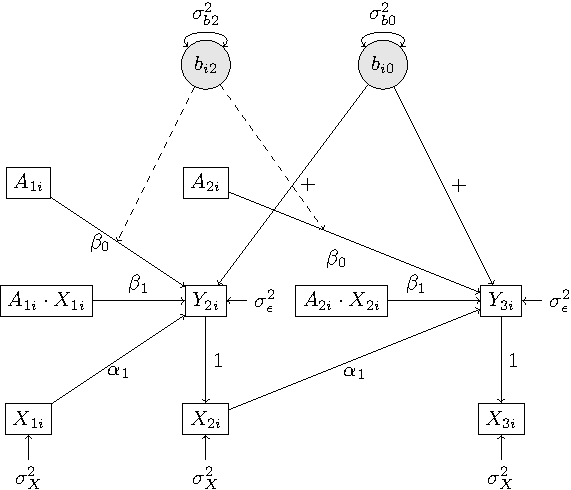
\includegraphics[width=0.9\textwidth,height=\textheight]{research-report_files/figure-pdf/fig-GM1_path-1.pdf}

}

\end{minipage}%
%
\begin{minipage}{0.50\linewidth}

\subcaption{\label{fig-GM3_path}GM3}

\centering{

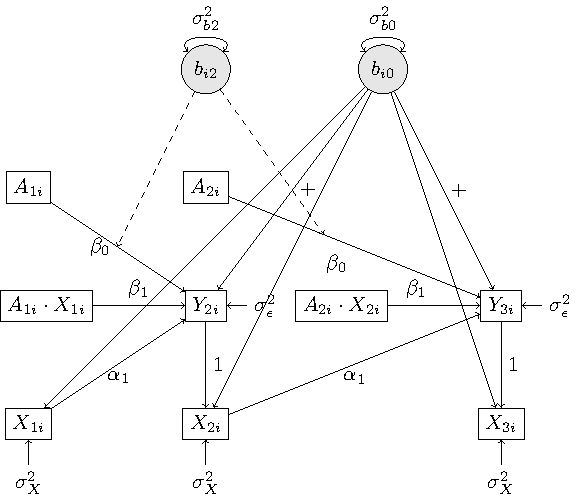
\includegraphics[width=0.9\textwidth,height=\textheight]{research-report_files/figure-pdf/fig-GM3_path-1.pdf}

}

\end{minipage}%
\newline
\begin{minipage}{0.50\linewidth}

\subcaption{\label{fig-GM3A_path}GM3A}

\centering{

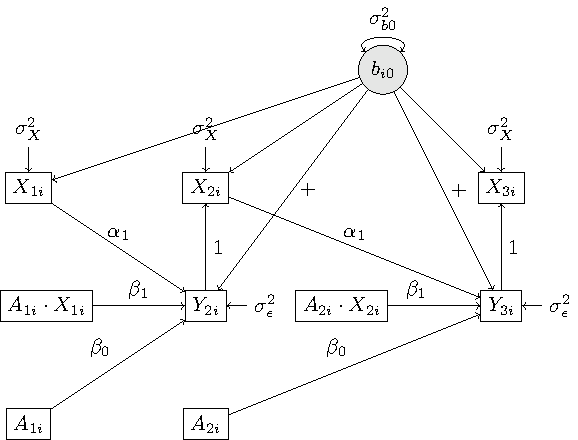
\includegraphics[width=0.9\textwidth,height=\textheight]{research-report_files/figure-pdf/fig-GM3A_path-1.pdf}

}

\end{minipage}%
%
\begin{minipage}{0.50\linewidth}

\subcaption{\label{fig-GM3B_path}GM3B}

\centering{

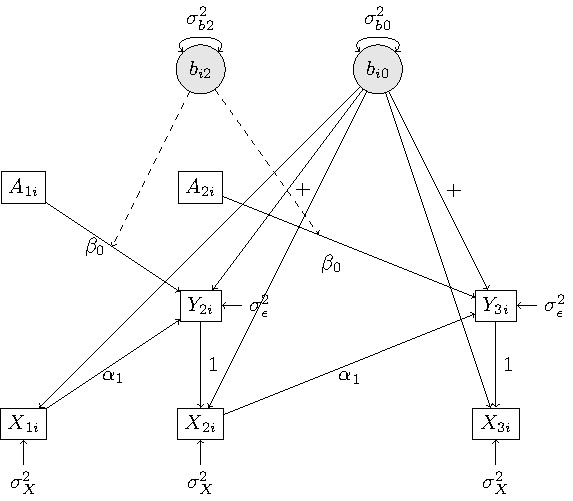
\includegraphics[width=0.9\textwidth,height=\textheight]{research-report_files/figure-pdf/fig-GM3B_path-1.pdf}

}

\end{minipage}%
\newline
\begin{minipage}{0.50\linewidth}
\emph{Note.} Random effects are represented by grey circles, observed
variables by squares and relationships across variables by arrows, where
dashed lines are reserved for random slopes.\end{minipage}%

\end{figure}%

\subsection{Backdoor Criterion and
DAGs}\label{backdoor-criterion-and-dags}

According to the backdoor criterion (\citeproc{ref-pearl1988}{Pearl,
1988}, \citeproc{ref-pearl2009}{2009}), a requirement for causal
identification, causal effects can be identified by blocking non-causal
paths through conditioning on intermediate variables (e.g., controlling
or matching). If any non-causal paths cannot be blocked due to omitted
variables or measurement error, treatment and outcome remain linked via
backdoor paths, leading to biased estimates of the treatment effect
(\citeproc{ref-Kim2021a}{Kim \& Steiner, 2021}).

DAGs are a useful tool for representing causal relationships between
variables and to evaluate the assumptions needed for causal
identification (see \citeproc{ref-elwert2014}{Elwert \& Winship, 2014}
for a psychological example). We formulated the DAGs for the first three
observations of each generative model, where the random disturbance
\(b_{0i}\) was represented by the node U (e.g.,
\citeproc{ref-Kim2021a}{Kim \& Steiner, 2021}, see
Figure~\ref{fig-DAGs}).

When applying Pearl's backdoor criterion to GM1/3/3A/3B, it may be
observed that there exists no backdoor path in the treatment effect
\(A_{it} \to Y_{it+1}\), as \(A_{it}\) does not have any parents. While
we need not control for covariate \(X_{it}\) to obtain an unbiased total
effect, doing so should not introduce bias. All things considered,
according to the backdoor criterion, controlling for the covariate
\(X_{it}\) should not result in biased estimates of the treatment effect
for any of the generative models.

\begin{figure}[H]

\caption{\label{fig-DAGs}DAGs for Generative Models 1, 3, 3A, 3B (t = 1,
2, 3)}

\begin{minipage}{0.50\linewidth}

\subcaption{\label{fig-GM1_DAG}GM 1}

\centering{

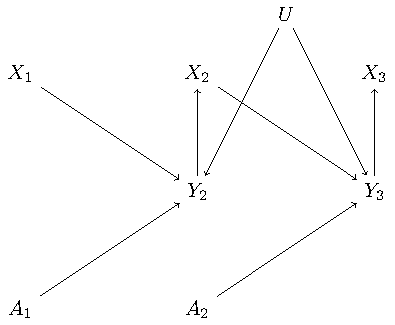
\includegraphics{research-report_files/figure-pdf/fig-GM1_DAG-1.pdf}

}

\end{minipage}%
%
\begin{minipage}{0.50\linewidth}

\subcaption{\label{fig-GM3_DAG}GM 3, 3A, 3B}

\centering{

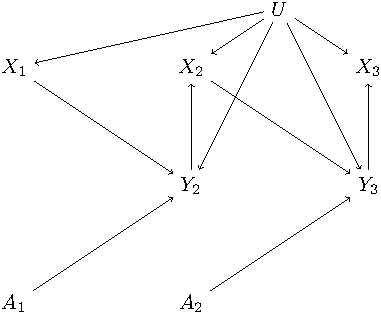
\includegraphics{research-report_files/figure-pdf/fig-GM3_DAG-1.pdf}

}

\end{minipage}%
\newline
\begin{minipage}{0.50\linewidth}
\emph{Note.} The red arrows show the biased backdoor path(s) in the
treatment efffect (before controlling for \(X_{it}\)).\end{minipage}%

\end{figure}%

\subsection{Data Analysis}\label{data-analysis}

We evaluated the performance of the models across a total of 24
different settings, each replicated 1,000 times, by systematically
varying the following factors:

\begin{itemize}
\item
  \textbf{Generative Models (GM):} 1, 3, 3A, 3B
\item
  \textbf{Number of timepoints (T):} 10, 30
\item
  \textbf{Sample size (N):} 30, 100, 200
\end{itemize}

All data generation and estimation was performed in \texttt{R}, version
4.4.2 (\citeproc{ref-rcoreteam2024}{Team, 2024}). After the generation
of data generation for any given setting, analytical multilevel linear
models were fit that are equivalent to each of the respective
data-generating models. To fit the standard MLM, the \texttt{lmer}
function from the R-package \texttt{lme4}
(\citeproc{ref-bates2015}{Bates et al., 2015}) was employed with
restricted maximum likelihood estimation.

\section{Results}\label{results}

Table~\ref{tbl-simulation-results} presents the simulation results for
each of the generative and analytical models. The estimates for the
analytical MLM may be interpreted in terms of bias, where given the
value of the treatment effect \(\beta_0 = 1\), absolute bias of .05
would imply \(5\%\) relative bias. Here we find the greatest absolute
bias of \(.02-.06\) for GM3, \(\leq .015\) for GM1/2, \(\leq .010\) for
GM3B and , \(\leq .005\) for GM3A. While the bias found for the original
GMs 1, 2 and 3 was slightly larger here compared to Qian et al.
(\citeproc{ref-qian2020}{2020}), the overall pattern remained the same.
To conclude, once we remove either the dependency of the random
intercept with the covariate (GM1), the random slope \(b_{i2}\) (GM3A)
or the interaction \(\beta_1\) (GM3B) from GM3, the bias dissapears or
becomes very small. The bias in GM3 decreases as the number of
timepoints \(T\) increases from 10 to 30. Note that the MLM model
fitting success rates are particularly poor for GM2, where in the worst
case, only 87 of the 1000 models were fitted.

\begin{table}

\caption{\label{tbl-simulation-results}Simulation results for Generative
Models 1, 2, 3, 3A and 3B over 1000 replications}

\centering{

\begin{tabu} to \linewidth {>{\raggedright\arraybackslash}p{5em}>{\raggedleft}X>{\raggedleft}X>{\raggedleft}X>{\raggedleft}X>{\raggedleft}X}
\toprule
\multicolumn{3}{c}{ } & \multicolumn{3}{c}{MLM} \\
\cmidrule(l{3pt}r{3pt}){4-6}
GM & T & N & Bias & SD & SR\\
\midrule
 &  & 30 & 0.000 & 0.238 & 0.998\\
\cmidrule{3-6}
 &  & 100 & -0.012 & 0.129 & 1.000\\
\cmidrule{3-6}
 & \multirow{-3}{*}{\raggedleft\arraybackslash 10} & 200 & 0.003 & 0.093 & 0.999\\
\cmidrule{2-6}
 &  & 30 & -0.001 & 0.203 & 0.998\\
\cmidrule{3-6}
 &  & 100 & -0.007 & 0.107 & 0.996\\
\cmidrule{3-6}
\multirow{-6}{5em}[0.5\dimexpr\aboverulesep+\belowrulesep+\cmidrulewidth]{\raggedright\arraybackslash 1} & \multirow{-3}{*}{\raggedleft\arraybackslash 30} & 200 & 0.001 & 0.079 & 0.996\\
\cmidrule{1-6}
 &  & 30 & 0.011 & 0.282 & 0.925\\
\cmidrule{3-6}
 &  & 100 & 0.005 & 0.147 & 0.881\\
\cmidrule{3-6}
 & \multirow{-3}{*}{\raggedleft\arraybackslash 10} & 200 & 0.008 & 0.103 & 0.844\\
\cmidrule{2-6}
 &  & 30 & 0.000 & 0.220 & 0.603\\
\cmidrule{3-6}
 &  & 100 & -0.014 & 0.114 & 0.247\\
\cmidrule{3-6}
\multirow{-6}{5em}[0.5\dimexpr\aboverulesep+\belowrulesep+\cmidrulewidth]{\raggedright\arraybackslash 2} & \multirow{-3}{*}{\raggedleft\arraybackslash 30} & 200 & -0.013 & 0.087 & 0.087\\
\cmidrule{1-6}
 &  & 30 & -0.052 & 0.245 & 0.999\\
\cmidrule{3-6}
 &  & 100 & -0.064 & 0.134 & 1.000\\
\cmidrule{3-6}
 & \multirow{-3}{*}{\raggedleft\arraybackslash 10} & 200 & -0.051 & 0.096 & 1.000\\
\cmidrule{2-6}
 &  & 30 & -0.024 & 0.206 & 0.997\\
\cmidrule{3-6}
 &  & 100 & -0.030 & 0.108 & 0.996\\
\cmidrule{3-6}
\multirow{-6}{5em}[0.5\dimexpr\aboverulesep+\belowrulesep+\cmidrulewidth]{\raggedright\arraybackslash 3} & \multirow{-3}{*}{\raggedleft\arraybackslash 30} & 200 & -0.023 & 0.080 & 0.997\\
\cmidrule{1-6}
 &  & 30 & 0.000 & 0.126 & 1.000\\
\cmidrule{3-6}
 &  & 100 & 0.004 & 0.073 & 1.000\\
\cmidrule{3-6}
 & \multirow{-3}{*}{\raggedleft\arraybackslash 10} & 200 & 0.002 & 0.048 & 1.000\\
\cmidrule{2-6}
 &  & 30 & -0.001 & 0.071 & 1.000\\
\cmidrule{3-6}
 &  & 100 & 0.000 & 0.040 & 1.000\\
\cmidrule{3-6}
\multirow{-6}{5em}[0.5\dimexpr\aboverulesep+\belowrulesep+\cmidrulewidth]{\raggedright\arraybackslash 3A} & \multirow{-3}{*}{\raggedleft\arraybackslash 30} & 200 & 0.000 & 0.028 & 1.000\\
\cmidrule{1-6}
 &  & 30 & 0.001 & 0.217 & 0.999\\
\cmidrule{3-6}
 &  & 100 & -0.008 & 0.121 & 1.000\\
\cmidrule{3-6}
 & \multirow{-3}{*}{\raggedleft\arraybackslash 10} & 200 & 0.005 & 0.087 & 1.000\\
\cmidrule{2-6}
 &  & 30 & 0.000 & 0.193 & 1.000\\
\cmidrule{3-6}
 &  & 100 & -0.008 & 0.103 & 0.997\\
\cmidrule{3-6}
\multirow{-6}{5em}[0.5\dimexpr\aboverulesep+\belowrulesep+\cmidrulewidth]{\raggedright\arraybackslash 3B} & \multirow{-3}{*}{\raggedleft\arraybackslash 30} & 200 & 0.001 & 0.075 & 0.999\\
\bottomrule
\end{tabu}

\emph{Note.} SR: model fitting success rate. Bias:
\(\hat{\beta}_{0,MLM} - \beta_{0,MLM}\). Difference:
\(\hat{\beta}_{0,GEE} - \beta_{0,MLM}\). SD: standard deviation of
estimates across replications.

}

\end{table}%

\section{Discussion}\label{discussion}

This report employed both graphical methods and data simulations to
understand and explain the issue of endogenous covariates. Now we first
discuss the expected results based on the backdoor criterion Pearl
(\citeproc{ref-pearl2009}{2009}) and the conditional independence
assumption (\citeproc{ref-qian2020}{Qian et al., 2020}), whereafter we
discuss the findings relating to the two research questions.

Using the conditional independence assumption of Qian et al.
(\citeproc{ref-qian2020}{2020}), we would expect, based on the path
diagrams, that the treatment effect would be biased for GM3, 3A and 3B.
On the other hand, the backdoor criterion suggested the absence of bias
for all generative models. While Qian et al.
(\citeproc{ref-qian2020}{2020}) show that GM3 is the only model with
bias in the treatment effect, the backdoor criterion failed to identify
this bias, as there is no backdoor path in the treatment effect. This
may be explained by the fact that the classic DAG does not impose
restrictions based on (a) the random slopes and (b) interaction effects.

The first research question---pertaining to the extent of treatment
effect bias in MLM estimates of generative model that were nested in
GM3---was investigated using the analytical multilevel model. First, we
reproduced the findings by Qian et al. (\citeproc{ref-qian2020}{2020})
who found consistent estimators for GM1 and and inconsistent ones for
GM3. Using additional generative models, we found that bias became
indiscernable when removing from GM3 either the dependency between the
random intercept and covariate (GM1), the random slope for treatment
(GM3A) or the interaction effect (GM3B). This finding is in sharp
contrast to the suggestion of the conditional independence assumption
that the treatment effect would be biased for GM3, 3A and 3B.

The current research report leaves several avenues unexplored. First, it
is unclear whether the simulation findings pertaining the generative
models in Qian et al. (\citeproc{ref-qian2020}{2020}) and here
generalize to other generative models. For instance, we found here that
removal of a random slope or interaction from GM3 got rid of most if not
all of the treatment effect bias. Thus, it is important to establish how
this generalizes, so that practical recommendations can be formulated.
This is particularly important, since while violations of model
assumptions are never desired, the robustness against and the practical
implications of a violation is what matters. Second, it is unclear how
exactly the divide between the literatures pertaining to the focus of
the MLM on different centering methods and within- and between-person
interpretations and the focus of the GEE on marginal and conditional
interpretations may be bridged. Consequently, future research could
assess the implications of centering methods in MLMs on the extent to
which the marginal interpretation of MLM breaks down. Third, we found
that the classical DAG may not be sufficient to identify bias in the
treatment effect for GM3, especially due to its lack of specification of
interaction effects. Concerns regarding the use of Pearl's backdoor
criterion in situations with interaction effects have been voiced by
several people (see Weinberg (\citeproc{ref-weinberg2007}{2007}); Attia
et al. (\citeproc{ref-attia2022}{2022})). Future research could explore
to what extent proposed extensions of the DAG may be useful in
identifying bias in the treatment effect for GM3. Finally, it may be
interesting to investigate the implications of endogenous covariates in
MLMs for other types of longitudinal data analysis methods, such as
dynamic structural equation modelling (DSEM; a widely used framework in
the social sciences based on MLM).

Third, since the issue extends to all longitudinal data analysis methods
according to Diggle (\citeproc{ref-diggle2002}{2002}), in future
research it may be interesting to investigate the implications of
endogenous covariates in MLMs for other types of longitudinal data
analysis methods, such as dynamic structural equation modelling (DSEM; a
widely used framework in the social sciences based on MLM).

\newpage

\section{References}\label{references}

\phantomsection\label{refs}
\begin{CSLReferences}{1}{0}
\bibitem[\citeproctext]{ref-attia2022}
Attia, J., Holliday, E., \& Oldmeadow, C. (2022). A proposal for
capturing interaction and effect modification using DAGs.
\emph{International Journal of Epidemiology}, \emph{51}(4), 1047--1053.
\url{https://doi.org/10.1093/ije/dyac126}

\bibitem[\citeproctext]{ref-bates2015}
Bates, D., Mächler, M., Bolker, B., \& Walker, S. (2015). Fitting linear
mixed-effects models using {lme4}. \emph{Journal of Statistical
Software}, \emph{67}(1), 148.
\url{https://doi.org/10.18637/jss.v067.i01}

\bibitem[\citeproctext]{ref-diggle2002}
Diggle, P. (2002). \emph{Analysis of Longitudinal Data}. OUP Oxford.

\bibitem[\citeproctext]{ref-elwert2014}
Elwert, F., \& Winship, C. (2014). Endogenous selection bias: The
problem of conditioning on a collider variable. \emph{Annual Review of
Sociology}, \emph{40}, 31--53.
\url{https://doi.org/10.1146/annurev-soc-071913-043455}

\bibitem[\citeproctext]{ref-hamaker2020}
Hamaker, E. L., \& Muthén, B. (2020). The fixed versus random effects
debate and how it relates to centering in multilevel modeling.
\emph{Psychological Methods}, \emph{25}(3), 365--379.
\url{https://doi.org/10.1037/met0000239}

\bibitem[\citeproctext]{ref-Kim2021a}
Kim, Y., \& Steiner, P. M. (2021). Causal graphical views of fixed
effects and random effects models. \emph{British Journal of Mathematical
and Statistical Psychology}, \emph{74}(2), 165--183.
\url{https://doi.org/10.1111/bmsp.12217}

\bibitem[\citeproctext]{ref-mcneish2017}
McNeish, D., Stapleton, L. M., \& Silverman, R. D. (2017). On the
unnecessary ubiquity of hierarchical linear modeling.
\emph{Psychological Methods}, \emph{22}(1), 114--140.
\url{https://doi.org/10.1037/met0000078}

\bibitem[\citeproctext]{ref-muth2016}
Muth, C., Bales, K. L., Hinde, K., Maninger, N., Mendoza, S. P., \&
Ferrer, E. (2016). Alternative Models for Small Samples in Psychological
Research: Applying Linear Mixed Effects Models and Generalized
Estimating Equations to Repeated Measures Data. \emph{Educational and
Psychological Measurement}, \emph{76}(1), 64--87.
\url{https://doi.org/10.1177/0013164415580432}

\bibitem[\citeproctext]{ref-pearl1988}
Pearl, J. (1988). \emph{Probabilistic Reasoning in Intelligent Systems:
Networks of Plausible Inference}. Morgan Kaufmann.

\bibitem[\citeproctext]{ref-pearl2009}
Pearl, J. (2009). \emph{Causality: Models, reasoning, and inference}
(2nd ed.). Cambridge University Press.

\bibitem[\citeproctext]{ref-qian2020}
Qian, T., Klasnja, P., \& Murphy, S. A. (2020). Linear mixed models with
endogenous covariates: Modeling sequential treatment effects with
application to a mobile health study. \emph{Statistical Science : A
Review Journal of the Institute of Mathematical Statistics},
\emph{35}(3), 375--390. \url{https://doi.org/10.1214/19-sts720}

\bibitem[\citeproctext]{ref-raudenbush2002}
Raudenbush, S. W., \& Bryk, A. S. (2002). \emph{Hierarchical Linear
Models: Applications and Data Analysis Methods} (2nd ed.). SAGE.

\bibitem[\citeproctext]{ref-rcoreteam2024}
Team, R. C. (2024). \emph{R: A language and environment for statistical
computing}. R Foundation for Statistical Computing.
\url{https://www.R-project.org/}

\bibitem[\citeproctext]{ref-weinberg2007}
Weinberg, C. R. (2007). Commentary: Can DAGs clarify effect
modification? \emph{Epidemiology}, \emph{18}(5), 569--572.
\url{https://www.jstor.org/stable/20486428}

\bibitem[\citeproctext]{ref-yan2013}
Yan, J., Aseltine, R. H., \& Harel, O. (2013). Comparing Regression
Coefficients Between Nested Linear Models for Clustered Data With
Generalized Estimating Equations. \emph{Journal of Educational and
Behavioral Statistics}, \emph{38}(2), 172--189.
\url{https://doi.org/10.3102/1076998611432175}

\end{CSLReferences}

~\textbar{} \textbar{} \textbar{} \textbar{} \textbar{}

\textbar---------------\textbar---------------\textbar---------------\textbar---------------\textbar---------------\textbar{}

Generative Model \textbar{} random slope treatment \(b_{i2}\) \textbar{}
interactie \(\beta_1\) \textbar{} fixed slope covariate \(\alpha_1\)
\textbar{} bias \textbar{}

3 \textbar{} yes \textbar{} yes \textbar{} yes \textbar{} yes, negative
\textbar{}

3a \textbar{} no \textbar{} yes \textbar{} yes \textbar{} no \textbar{}

3d \textbar{} yes \textbar{} no \textbar{} yes \textbar{} no \textbar{}

3h \textbar{} yes \textbar{} yes \textbar{} no \textbar{} yes, positive
\textbar{}

: Models with 1 Parameter Less




\end{document}
